% Lab 2 DQN report. Compile with XeLaTeX (or Tectonic):  tectonic report.tex
% Figures are read from figures/ (training curves) and screenshot/ (test results).
\documentclass[11pt,a4paper]{article}

\usepackage[margin=2.2cm]{geometry}
\usepackage{fontspec}
\usepackage{xeCJK}
% Tectonic cannot read C:/Windows/Fonts directly, so the font files are copied
% into .fonts/. Without them, fall back to the installed font by name
% (MiKTeX / TeX Live on Windows). On Overleaf, replace with e.g. {Noto Serif CJK TC}.
\IfFileExists{.fonts/msjh.ttc}{
  \setCJKmainfont{msjh.ttc}[Path=.fonts/, BoldFont=msjhbd.ttc]
  \setCJKsansfont{msjh.ttc}[Path=.fonts/, BoldFont=msjhbd.ttc]
  \setCJKmonofont{msjh.ttc}[Path=.fonts/]
}{
  \setCJKmainfont{Microsoft JhengHei}
  \setCJKsansfont{Microsoft JhengHei}
  \setCJKmonofont{Microsoft JhengHei}
}
\xeCJKsetup{CJKecglue={\hskip 0.15em plus 0.05em}}

\usepackage{amsmath}
\usepackage{graphicx}
\usepackage{booktabs}
\usepackage{array}
\usepackage{needspace}
\usepackage{float}
\usepackage{caption}
\usepackage{listings}
\usepackage{xcolor}
\usepackage{enumitem}
\usepackage[hidelinks]{hyperref}

\captionsetup{font=small, labelfont=bf}
\setlist{itemsep=2pt, topsep=4pt}
\renewcommand{\arraystretch}{1.15}
\setlength{\parindent}{0pt}
\setlength{\parskip}{4pt}

\lstset{
  language=Python,
  basicstyle=\ttfamily\small,
  keywordstyle=\color{blue!70!black},
  commentstyle=\color{green!45!black},
  frame=single, rulecolor=\color{gray!50},
  backgroundcolor=\color{gray!6},
  columns=fullflexible, breaklines=true,
  xleftmargin=4pt, xrightmargin=4pt,
}

% Two figures side by side.
\newcommand{\pair}[4]{%
  \begin{figure}[H]\centering
  \begin{minipage}{0.49\linewidth}\centering
    \includegraphics[width=\linewidth]{#1}\\[-2pt]{\small #2}
  \end{minipage}\hfill
  \begin{minipage}{0.49\linewidth}\centering
    \includegraphics[width=\linewidth]{#3}\\[-2pt]{\small #4}
  \end{minipage}
  \end{figure}}

% One test-result screenshot.
\newcommand{\testshot}[1]{%
  \begin{figure}[H]\centering
  \includegraphics[width=0.72\linewidth]{#1}
  \end{figure}}

\title{\textbf{Lab 2: Deep Q-Network (DQN) 實驗報告}}
\author{}
\date{}

\begin{document}
\maketitle

%======================================================================
\section{實作概要}

\subsection{環境前處理（Atari 常用技巧）}

\begin{table}[H]\centering\small
\begin{tabular}{>{\raggedright\arraybackslash}p{2.6cm}>{\raggedright\arraybackslash}p{4.2cm}>{\raggedright\arraybackslash}p{7.8cm}}
\toprule
技巧 & 設定 & 說明 \\
\midrule
Frame skip & 4 & \texttt{gym.make(frameskip=1)} 搭配 \texttt{AtariPreprocessing(frame\_skip=4)}，只跳一次，避免 v5 預設的 frameskip 與 wrapper 疊成 16 \\
Max-pooling & 取最後兩幀逐像素 max & 消除 Atari 精靈閃爍 \\
Grayscale + Resize & $210\times160\times3 \rightarrow 84\times84$ & 降低輸入維度 \\
Frame stack & 4 幀 & 讓網路從靜態影像推出速度與方向 \\
Reward clipping & 訓練用 reward 裁到 $[-1,1]$ & 只影響寫入 replay buffer 的值；TensorBoard 記錄的是原始分數 \\
Sticky actions & 0.25（v5 預設） & 保留官方 benchmark 設定 \\
\bottomrule
\end{tabular}
\end{table}

\subsection{網路架構}

使用 DeepMind Nature DQN：輸入 $(4,84,84)$ 除以 255 後，依序經過
Conv(32, $8\times8$, stride 4) $\rightarrow$ Conv(64, $4\times4$, stride 2) $\rightarrow$ Conv(64, $3\times3$, stride 1)，
每層後接 ReLU，攤平成 3136 維，再經 FC(512)--ReLU--FC($|A|$) 輸出各動作的 Q 值。

Dueling DQN 共用同樣的卷積層，把最後的全連接層拆成價值 $V(s)$ 與優勢 $A(s,a)$ 兩支（各為 FC(512)--ReLU--FC），再組合為
\[
Q(s,a) = V(s) + \Big( A(s,a) - \frac{1}{|A|}\sum_{a'} A(s,a') \Big).
\]

\subsection{DQN 更新流程}

\begin{itemize}
  \item \textbf{Epsilon-greedy}：以機率 $\varepsilon$ 隨機選動作，否則取 $\arg\max_a Q(s,a;\theta)$。$\varepsilon$ 在前 1M 步從 1.0 線性降到 0.1，直接由步數算出，不逐步遞減。
  \item \textbf{Experience replay}：容量 100{,}000。每個 transition 只存一張 $84\times84$ uint8 影格，抽樣時再依索引重建 4 幀堆疊，記憶體約 0.7\,GB（直接存 state/next\_state 約 5.6\,GB）。
  \item \textbf{Q 值與 target}（\texttt{src/dqn\_agent\_atari.py}）：
\end{itemize}

\noindent\begin{minipage}{\linewidth}
\begin{lstlisting}
q_value = self.behavior_net(state).gather(1, action.unsqueeze(1)).squeeze(1)
with torch.no_grad():
    if self.double:   # DDQN: online net picks the action, target net scores it
        next_action = self.behavior_net(next_state).argmax(dim=1, keepdim=True)
        q_next = self.target_net(next_state).gather(1, next_action).squeeze(1)
    else:             # DQN: target net both picks and scores
        q_next = self.target_net(next_state).max(dim=1).values
    q_target = reward + self.gamma * q_next * (1.0 - done)
loss = self.criterion(q_value, q_target)   # MSE, as in the handout pseudocode
\end{lstlisting}
\end{minipage}

\begin{itemize}
  \item \textbf{網路更新}：每 4 個 env step 對 behavior network 做一次梯度下降（Adam），每 10{,}000 步把 behavior network 的權重複製到 target network。
  \item \texttt{done} 只在遊戲真正結束（terminated）時為 1。因時間上限被截斷（truncated）的 episode 仍會 bootstrap，因為最後的狀態不是終止狀態。
\end{itemize}

\subsection{超參數}

\begin{table}[H]\centering\small
\begin{tabular}{ll}
\toprule
參數 & 值 \\
\midrule
Replay buffer 容量 & 100{,}000 \\
Batch size & 32 \\
Warmup steps & 20{,}000 \\
Optimizer & Adam（lr = $6.25\times10^{-5}$，eps = $1.5\times10^{-4}$） \\
Epsilon & 1.0 $\rightarrow$ 0.1（線性，1M 步） \\
Gamma & 0.99 \\
Behavior network 更新頻率 & 每 4 步 \\
Target network 更新頻率 & 每 10{,}000 步 \\
Loss & MSE \\
Gradient norm clipping & 10.0 \\
評估 & 每 100k 步評估 5 場完整遊戲，$\varepsilon=0.01$，固定 seed 10000--10004 \\
測試 & 用 \texttt{best.pt} 跑 5 場完整遊戲，$\varepsilon=0.01$，seed 0--4 \\
\bottomrule
\end{tabular}
\end{table}

五組實驗都用 seed 0，每組相對 DQN baseline 只改一個條件。五組在同一張 RTX 2080 Ti 上同時訓練。

圖中淡色線是原始數值，實線是與 TensorBoard 相同算法的 EMA 平滑（weight 0.9）。x 軸是累積 env steps；平行化 rollout 的步數是 8 個環境的總和。

%======================================================================
\section{DQN — MsPacman-v5}

訓練 20M env steps，耗時 17.5 小時。

\subsection{Training curve}
\pair{figures/MsPacman_dqn__Train_Episode_Reward.png}{Train/Episode Reward}
     {figures/MsPacman_dqn__Evaluate_Episode_Reward.png}{Evaluate/Episode Reward}
\pair{figures/MsPacman_dqn__Train_Q_Mean.png}{Train/Q Mean}
     {figures/MsPacman_dqn__Train_Loss.png}{Train/Loss}

\subsection{Testing results（5 games）}
\testshot{screenshot/MsPacman_dqn_test_result.png}

\subsection{觀察}
\begin{itemize}
  \item \textbf{學習速度}：評估分數 0.42M 步第一次超過 1000，3.12M 步超過 2000，之後成長明顯變慢。各區間的評估平均：0--2M 為 967，2--5M 為 1778，5--10M 為 2178，10--20M 為 2317。
  \item \textbf{後半段幾乎停滯}：後 10M 步的平均只比前一段多約 140 分。單次最高評估 4044 出現在 14.32M 步，但平滑曲線在那段只有約 2400，屬於 5 場評估的雜訊尖峰。最後一次評估（19.92M 步）是 2548。
  \item \textbf{\texttt{best.pt} 的選擇偏差}：\texttt{best.pt} 是評估平均最高（4044）的 checkpoint，但換 seed 測試只得 2954。用單次 5 場的最高值挑模型，會偏向挑到運氣好的那一次。
  \item \textbf{Q 值}：Train/Q Mean 在約 2.5M 步升到約 20，之後在 10--20M 步緩慢降到約 17。這裡的 Q 是在 clipped reward 尺度下。
\end{itemize}

%======================================================================
\section{DQN — Enduro-v5}

訓練 10M env steps，耗時 12.8 小時。

\subsection{Training curve}
\pair{figures/Enduro_dqn__Train_Episode_Reward.png}{Train/Episode Reward}
     {figures/Enduro_dqn__Evaluate_Episode_Reward.png}{Evaluate/Episode Reward}

\subsection{Testing results（5 games）}
\testshot{screenshot/Enduro_dqn_test_result.png}

\subsection{觀察}
\begin{itemize}
  \item \textbf{前約 1M 步 reward 幾乎都是 0}：Enduro 要超車才會得分，而前 1M 步 $\varepsilon$ 還在從 1.0 往下降，隨機動作很難持續加速並超車，agent 長時間拿不到非零的回饋。$\varepsilon$ 降低、agent 開始穩定前進後，reward 在 1--2M 步之間快速上升。
  \item \textbf{還沒收斂}：評估平均在 5--10M 步是 662，最後 1M 步是 821。最佳評估 1142 出現在 9.32M 步，接近訓練結束，曲線仍在上升，再多訓練應該還會進步。
  \item \textbf{測試}：5 場中有 4 場打完約 13{,}300 步、分數在 1030--1090。第 3 場只有一半長度、分數也只有一半（484），推測是某一天沒達到超車門檻，遊戲提前結束。
\end{itemize}

%======================================================================
\section{DDQN vs DQN}

DDQN 只改 target 的計算：$y = r + \gamma\, Q_{\text{target}}\big(s', \arg\max_{a'} Q_{\text{online}}(s',a')\big)$，網路與其他設定都和 DQN 相同。訓練 10M 步。

\subsection{Training curve（comparison）}
\pair{figures/compare__dqn_vs_ddqn__Evaluate_Episode_Reward.png}{Evaluate/Episode Reward}
     {figures/compare__dqn_vs_ddqn__Train_Episode_Reward.png}{Train/Episode Reward}
\begin{figure}[H]\centering
  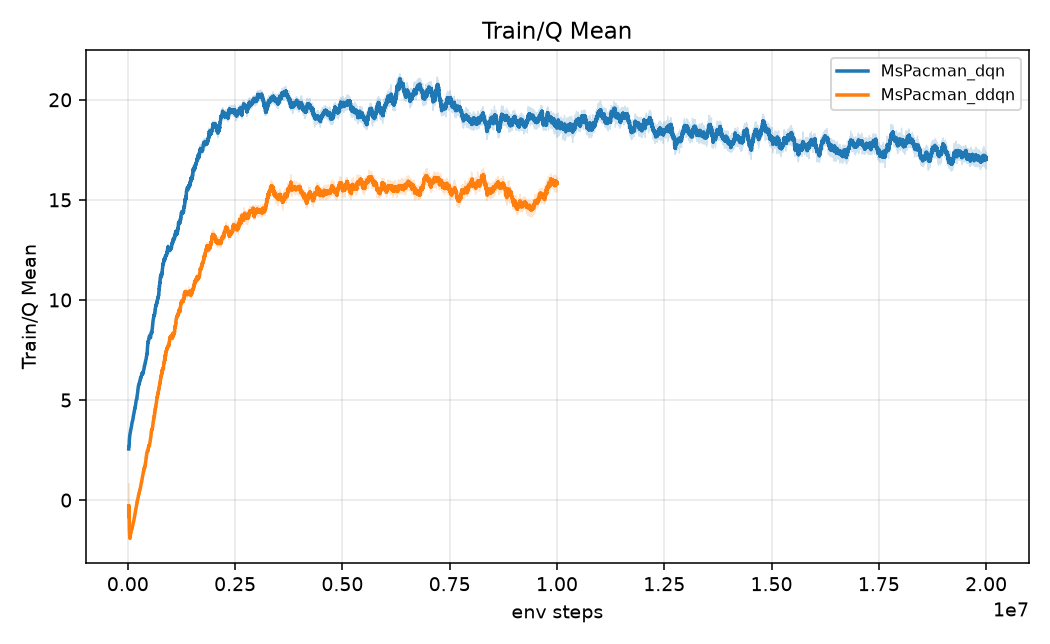
\includegraphics[width=0.55\linewidth]{figures/compare__dqn_vs_ddqn__Train_Q_Mean.png}\\[-2pt]
  {\small Train/Q Mean}
\end{figure}

\subsection{Testing results（5 games）}
\testshot{screenshot/MsPacman_ddqn_test_result.png}

\subsection{比較（同樣 10M 步內）}
\begin{table}[H]\centering\small
\begin{tabular}{lll}
\toprule
指標 & DQN & DDQN \\
\midrule
評估平均，5--10M 步 & 2178 & \textbf{2284} \\
評估平均，9--10M 步 & 2106 & \textbf{2451} \\
最佳評估（$\le$10M） & 2866 & \textbf{3444} \\
第一次評估 $\ge$ 2000 & 3.12M 步 & \textbf{1.32M 步} \\
第一次評估 $\ge$ 3000 & 10.02M 步 & \textbf{5.32M 步} \\
Train/Q Mean，5--10M 步 & 19.5 & \textbf{15.5} \\
\texttt{best.pt} 測試平均（seed 0--4） & 2954（20M 步的模型） & \textbf{3502} \\
51 個 seed 中單場 $>$ 3000 的數量 & 10 / 51（20M 步的模型） & \textbf{25 / 51} \\
\bottomrule
\end{tabular}
\end{table}

\subsection{討論}
\begin{itemize}
  \item \textbf{Over-estimation}：DQN 的 target $\max_{a'} Q_{\text{target}}(s',a')$ 用同一個網路選動作又估值。Q 的估計有雜訊時，取 max 會偏向剛好被高估的動作，所以 target 系統性偏高，而且這個偏差會透過 bootstrap 一路傳下去。DDQN 讓 online 網路選動作、target 網路估值，選擇和評估的雜訊不再是同一份，max 帶來的正向偏差因此變小。
  \item \textbf{實驗結果與此一致}：DDQN 的 Q 值在整段訓練都比 DQN 低約 4（5--10M 步 15.5 vs 19.5，約低 20\%）。DQN 的 Q 值在約 6M 步達到約 21 後逐步下降，DDQN 則一直穩定在 15--16。不過要注意，Dueling DQN 用的是 DQN target，它的 Q 值卻也在 15.5 左右（見第 5 節），所以兩者 Q 值的差距不能全部歸因於 over-estimation。要直接證明高估，需要把 Q 和實際的折扣回報比較，這次沒有量。
  \item \textbf{表現}：DDQN 達到 2000 和 3000 分所需的步數都只有 DQN 的一半左右，10M 步內的最佳評估也高出約 580。最終模型在 demo 上也最穩：51 個 seed 中有一半單場超過 3000，DQN 只有五分之一。
  \item \textbf{限制}：每種方法只跑了一個 seed，單次評估的標準差在 600--1400 之間，DQN 與 DDQN 的平滑曲線在 3--8M 步之間有很長一段幾乎重疊。這些差距符合理論預期，但不能視為統計上確定的結論。
\end{itemize}

%======================================================================
\section{Dueling DQN vs DQN}

Dueling DQN 只改網路架構（見 1.2 節），target 仍是 DQN 的寫法。訓練 10M 步。

\subsection{Training curve（comparison）}
\pair{figures/compare__dqn_vs_dueling__Evaluate_Episode_Reward.png}{Evaluate/Episode Reward}
     {figures/compare__dqn_vs_dueling__Train_Episode_Reward.png}{Train/Episode Reward}
\begin{figure}[H]\centering
  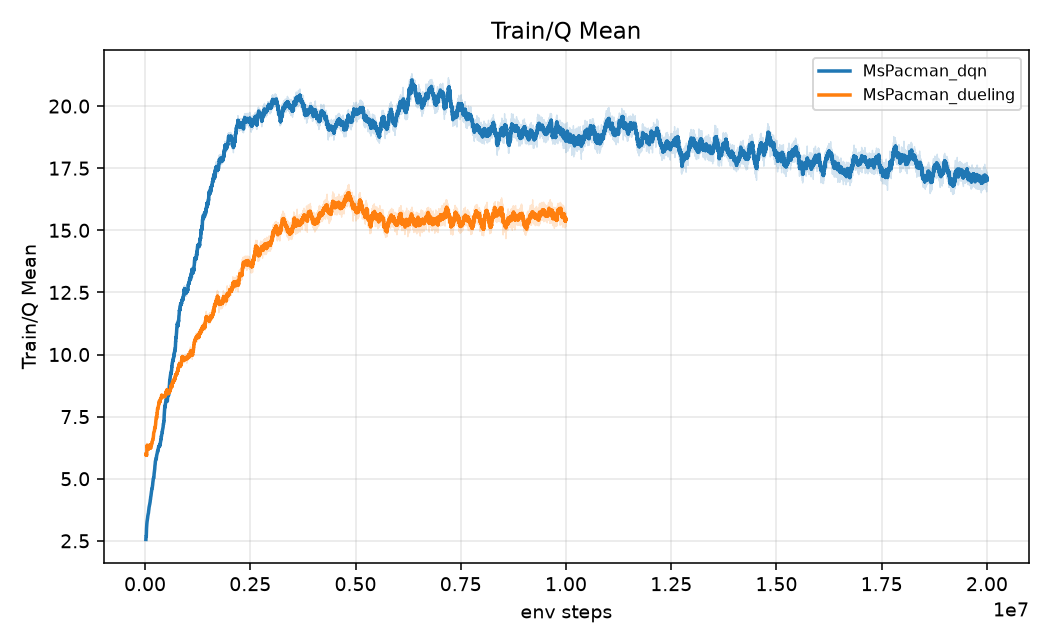
\includegraphics[width=0.55\linewidth]{figures/compare__dqn_vs_dueling__Train_Q_Mean.png}\\[-2pt]
  {\small Train/Q Mean}
\end{figure}

\subsection{Testing results（5 games）}
\testshot{screenshot/MsPacman_dueling_test_result.png}

\subsection{比較（同樣 10M 步內）}
\begin{table}[H]\centering\small
\begin{tabular}{lll}
\toprule
指標 & DQN & Dueling \\
\midrule
評估平均，0--2M 步 & 967 & \textbf{1102} \\
第一次評估 $\ge$ 1000 & 0.42M 步 & \textbf{0.32M 步} \\
評估平均，2--5M 步 & 1778 & 1777 \\
評估平均，5--10M 步 & \textbf{2178} & 1892 \\
最佳評估（$\le$10M） & \textbf{2866} & 2286（4.02M 步） \\
Train/Q Mean，5--10M 步 & 19.5 & 15.5 \\
\texttt{best.pt} 測試平均（seed 0--4） & \textbf{2954}（20M 步的模型） & 2072 \\
模型大小 & 27 MB & 53 MB \\
\bottomrule
\end{tabular}
\end{table}

\subsection{討論}
\begin{itemize}
  \item \textbf{架構差異}：Dueling 把 Q 拆成狀態價值 $V(s)$ 和動作優勢 $A(s,a)$。在 MsPacman 裡，很多狀態（例如在直線走道、附近沒有鬼）不管選哪個動作，結果都差不多。DQN 每次更新只修正被選到的那一個 $Q(s,a)$，Dueling 則每次都會更新共用的 $V(s)$，所以狀態價值學得比較快，需要學的也只剩動作之間的相對差異。減掉 advantage 的平均是為了讓 $V$ 和 $A$ 可以唯一分解，否則常數可以在兩者之間任意移動。
  \item \textbf{前期學得較快}：這和上面的說法一致。Dueling 是三者中最早到 1000 分的（0.32M 步），0--2M 步的評估平均也比 DQN 高約 135。
  \item \textbf{後期停在較低的水準}：從約 4M 步開始，Dueling 的評估平均就停在約 1900，最佳評估 2286 出現在 4.02M 步，後面 6M 步都沒有再超過；DQN 則繼續升到約 2200。可能的原因：
  \begin{enumerate}
    \item 全連接層從一支變兩支，參數幾乎多了一倍（53 MB vs 27 MB），但學習率和 gradient clipping 都沿用 DQN 的設定。原論文會把回傳到卷積層的梯度乘上 $1/\sqrt{2}$，並調整學習率，這次沒有做。
    \item 只跑一個 seed，前期優勢和後期劣勢都可能在 seed 變異的範圍內。
  \end{enumerate}
  \item \textbf{Q 值}：Dueling 的 Q 值也穩定在 15.5 左右，比 DQN 低，跟 DDQN 差不多，但它用的是 DQN target。這表示網路架構本身也會改變 Q 值的大小，所以不能只看 Q 值高低就判斷高估的程度。
\end{itemize}

%======================================================================
\section{DQN with parallelized rollout vs DQN}

用 8 個 \texttt{AsyncVectorEnv} 環境同時收集資料，演算法與超參數完全不變：
\begin{itemize}
  \item 每 4 個 env step（8 個環境的總和）一次梯度更新，所以兩者在同樣 env steps 下的梯度更新次數相同。
  \item Replay buffer 總容量仍是 100{,}000，切成 8 段、每段 12{,}500，每個環境寫自己那段，避免不同 episode 的影格交錯、破壞 frame stack。
  \item Target network 同步改用計數器判斷是否跨過 10{,}000 步，因為步數一次跳 8，用 \texttt{step \% 10000 == 0} 可能永遠不會觸發。
\end{itemize}
訓練 10M 步。

\subsection{Training curve（comparison）}
以 env steps 為 x 軸（樣本效率）：
\pair{figures/compare__dqn_vs_parallel__Evaluate_Episode_Reward.png}{Evaluate/Episode Reward}
     {figures/compare__dqn_vs_parallel__Train_Episode_Reward.png}{Train/Episode Reward}
以 wall-clock 時間為 x 軸（實際花費時間）：
\pair{figures/compare__dqn_vs_parallel__Evaluate_Episode_Reward__wall.png}{Evaluate/Episode Reward（wall-clock）}
     {figures/compare__dqn_vs_parallel__Perf_Steps_Per_Second.png}{Perf/Steps Per Second}

\subsection{Testing results（5 games）}
\testshot{screenshot/MsPacman_parallel_test_result.png}

\subsection{比較}
\begin{table}[H]\centering\small
\begin{tabular}{lll}
\toprule
指標 & DQN（1 env） & Parallel（8 envs） \\
\midrule
吞吐量（五組同時訓練） & 316 步/秒 & \textbf{374 步/秒}（1.18$\times$） \\
吞吐量（單獨跑，50k 步 smoke test） & 約 560 步/秒 & \textbf{約 725 步/秒}（約 1.3$\times$） \\
跑完 10M 步的時間 & 約 11.1 h & \textbf{7.4 h} \\
第一次評估 $\ge$ 2000 & 3.12M 步 / 3.55 h & 1.92M 步 / \textbf{1.41 h} \\
評估平均，5--10M 步 & \textbf{2178} & 1930 \\
評估平均，9--10M 步 & 2106 & \textbf{2138} \\
最佳評估（$\le$10M） & \textbf{2866} & 2848（2.02M 步） \\
\texttt{best.pt} 測試平均（seed 0--4） & \textbf{2954}（20M 步的模型） & 1580 \\
\bottomrule
\end{tabular}
\end{table}

\subsection{討論}
\begin{itemize}
  \item \textbf{主要差異是牆鐘時間}：DQN 單環境時，每一步都要依序做「環境模擬 $\rightarrow$ 網路推論 $\rightarrow$ 存入 buffer」。平行化後，8 個環境在不同 process 同時模擬，推論也合成一個 batch，平均到每步的成本就降低了。在同樣的 7.4 小時內，平行化版本跑完 10M 步，單環境版本只跑到約 6.3M 步。以時間為 x 軸時，平行化曲線在 1--4 小時之間明顯領先，例如 1.41 小時就到 2000 分，DQN 要 3.55 小時。
  \item \textbf{加速遠不到 8 倍}：因為我們保持「每 4 個 env step 一次更新」，梯度更新的次數只和總步數有關，與環境數量無關。平行化只加速了資料收集，梯度更新（batch 32 的前向、反向傳播）一點都沒變少。加上這次五組實驗共用一張 GPU（使用率約 98\%），GPU 才是瓶頸，所以加速比從單獨跑的約 1.3$\times$ 進一步縮小到 1.18$\times$。
  \item \textbf{樣本效率略差或相當}：用 env steps 比較時，兩條曲線大致重疊。5--10M 步的平均平行化低約 250，但最後 1M 步兩者相當（2138 vs 2106）。平行化時，8 個環境在同一組參數下各跑 8 步之後才會再更新，資料和當前 policy 的距離稍微大一點，這可能讓樣本效率略低。
  \item \textbf{測試分數偏低的原因}：平行化版本的最佳評估（2848）出現在很早的 2.02M 步，是一次雜訊尖峰，所以 \texttt{best.pt} 其實是一個只訓練 2M 步的模型，換 seed 測試只剩 1580。從評估曲線看，平行化版本在 9--10M 步的表現（約 2140）比 \texttt{best.pt} 還好。這是「用單次 5 場評估挑 checkpoint」的問題，和平行化本身無關。
\end{itemize}

%======================================================================
\section{總結}

\begin{table}[H]\centering\small
\begin{tabular}{llrrrrr}
\toprule
實驗 & 環境 & 步數 & 耗時 & 最佳評估 & 測試平均 & 測試單場最高 \\
\midrule
DQN & MsPacman & 20M & 17.5 h & 4044 & 2954 & 4960 \\
DQN & Enduro & 10M & 12.8 h & 1142 & 948.8 & 1094 \\
DDQN & MsPacman & 10M & 11.3 h & 3444 & \textbf{3502} & \textbf{5050} \\
Dueling DQN & MsPacman & 10M & 12.7 h & 2286 & 2072 & 2270 \\
DQN（8 envs） & MsPacman & 10M & 7.4 h & 2848 & 1580 & 2530 \\
\bottomrule
\end{tabular}
\end{table}

\begin{itemize}
  \item 在這次的設定中，\textbf{DDQN 是 MsPacman 上表現最好的方法}：只用 DQN 一半的步數，測試平均和穩定度都比較好。
  \item Dueling 前期學得較快，但後期停在較低的分數。平行化 rollout 主要節省的是牆鐘時間，不提升樣本效率。
  \item 所有比較都只有一個 seed，且評估雜訊大（單次 5 場的標準差 600--1400），結論應視為趨勢而非定論。
\end{itemize}

\subsection*{Demo 模型}
用 \texttt{find\_best\_seed.py} 掃描 seed 0--50 後，demo 選用 \texttt{MsPacman\_ddqn/best.pt}、\textbf{seed 18，單場 5310 分}。同一個 checkpoint 和同一個 seed 會重現完全相同的遊戲（ALE reset、sticky actions、隨機 no-op、epsilon 擲骰都由同一個 seed 決定）。

\begin{lstlisting}[language=bash]
cd src
python test.py --checkpoint ../checkpoints/MsPacman_ddqn/best.pt --seeds 18 --episodes 1 --record-video
\end{lstlisting}

%======================================================================
\needspace{8\baselineskip}
\section*{References}
\begin{enumerate}[label={[\arabic*]}]
  \item V. Mnih et al. ``Playing Atari with Deep Reinforcement Learning.'' arXiv:1312.5602, 2013.
  \item V. Mnih et al. ``Human-level control through deep reinforcement learning.'' \textit{Nature} 518, 2015.
  \item H. van Hasselt, A. Guez, D. Silver. ``Deep Reinforcement Learning with Double Q-Learning.'' AAAI, 2016.
  \item Z. Wang et al. ``Dueling Network Architectures for Deep Reinforcement Learning.'' ICML, 2016.
\end{enumerate}

\end{document}
